\subsubsection{Nutzwertanalyse}Zur Auswertung wurde eine Nutzwertanalyse durchgeführt, bei der die Primärkriterien auf Erfüllung oder Nichterfüllung hin geprüft wurden. Idealerweisen sollten dabei alle Primärziele erfüllt werden. Alle anderen Ziele wurden gemäss Tabelle \ref{tab:zielgewichtung} neu gewichtet und deren Erfüllung mit einer Note von 1 bis 10 und bei Nichterfüllung 0 bewertet. Die Multiplikation der Gewichtuung mit der Note ergibt ein Zwischenresultat für ein Ziel. Die Summe der Zwischenresultate ergibt die Gesamtpunktzahl nach Sekundärzielen. Diese Analyse ist in Abbildung \ref{pic:nutzwertanalyse} dargestellt. Mit diesen Kriterien erfüllt nur \textbf{Variante D} die Muss-Ziele.
\subsubsection{Kosten-Nutzen Analyse}
In Bezug zu den verwendeten Komponenten und Materialien kann eine Schätzung für die Kosten jeder Variante abgegeben werden:
\begin{itemize}
	\item \textbf{Variante A: Alles Analog}: Hoch, vor allem durch den Zeitaufwand
	\item \textbf{Variante B: Drahtlos \& Portabel}: Mittel, jedoch PMMA als Preistreiber
	\item \textbf{Variante C: High-End Audiophil}: Sehr hoch, durch Spezial- und High-End Komponenten
	\item \textbf{Variante D: Einfache Anwendung, Plug’n’Play}: Tief-Mittel
	\item \textbf{Variante E: Neu ist besser}: Mittel, jedoch PMMA und Zeitaufwand
\end{itemize}
Diese Erkenntnis kann auf die in der Nutzwertanalyse erreichte Punktzahl abgebildet werden. Abbildung \ref{pic:kostennutzen} zeigt dieses Verhältnis grafisch auf. Dabei sind Lösung mit Tendenz in Richtung untere rechte Ecke (\textit{hoher Nutzen, tiefe Kosten}) zu bevorzugen. Dagegen sind Lösungen mit Tendenz Richtung oberen linke Ecke mit hohen Kosten, aber wenig Nutzen verbunden.
\begin{figure}[H]
	\centering
	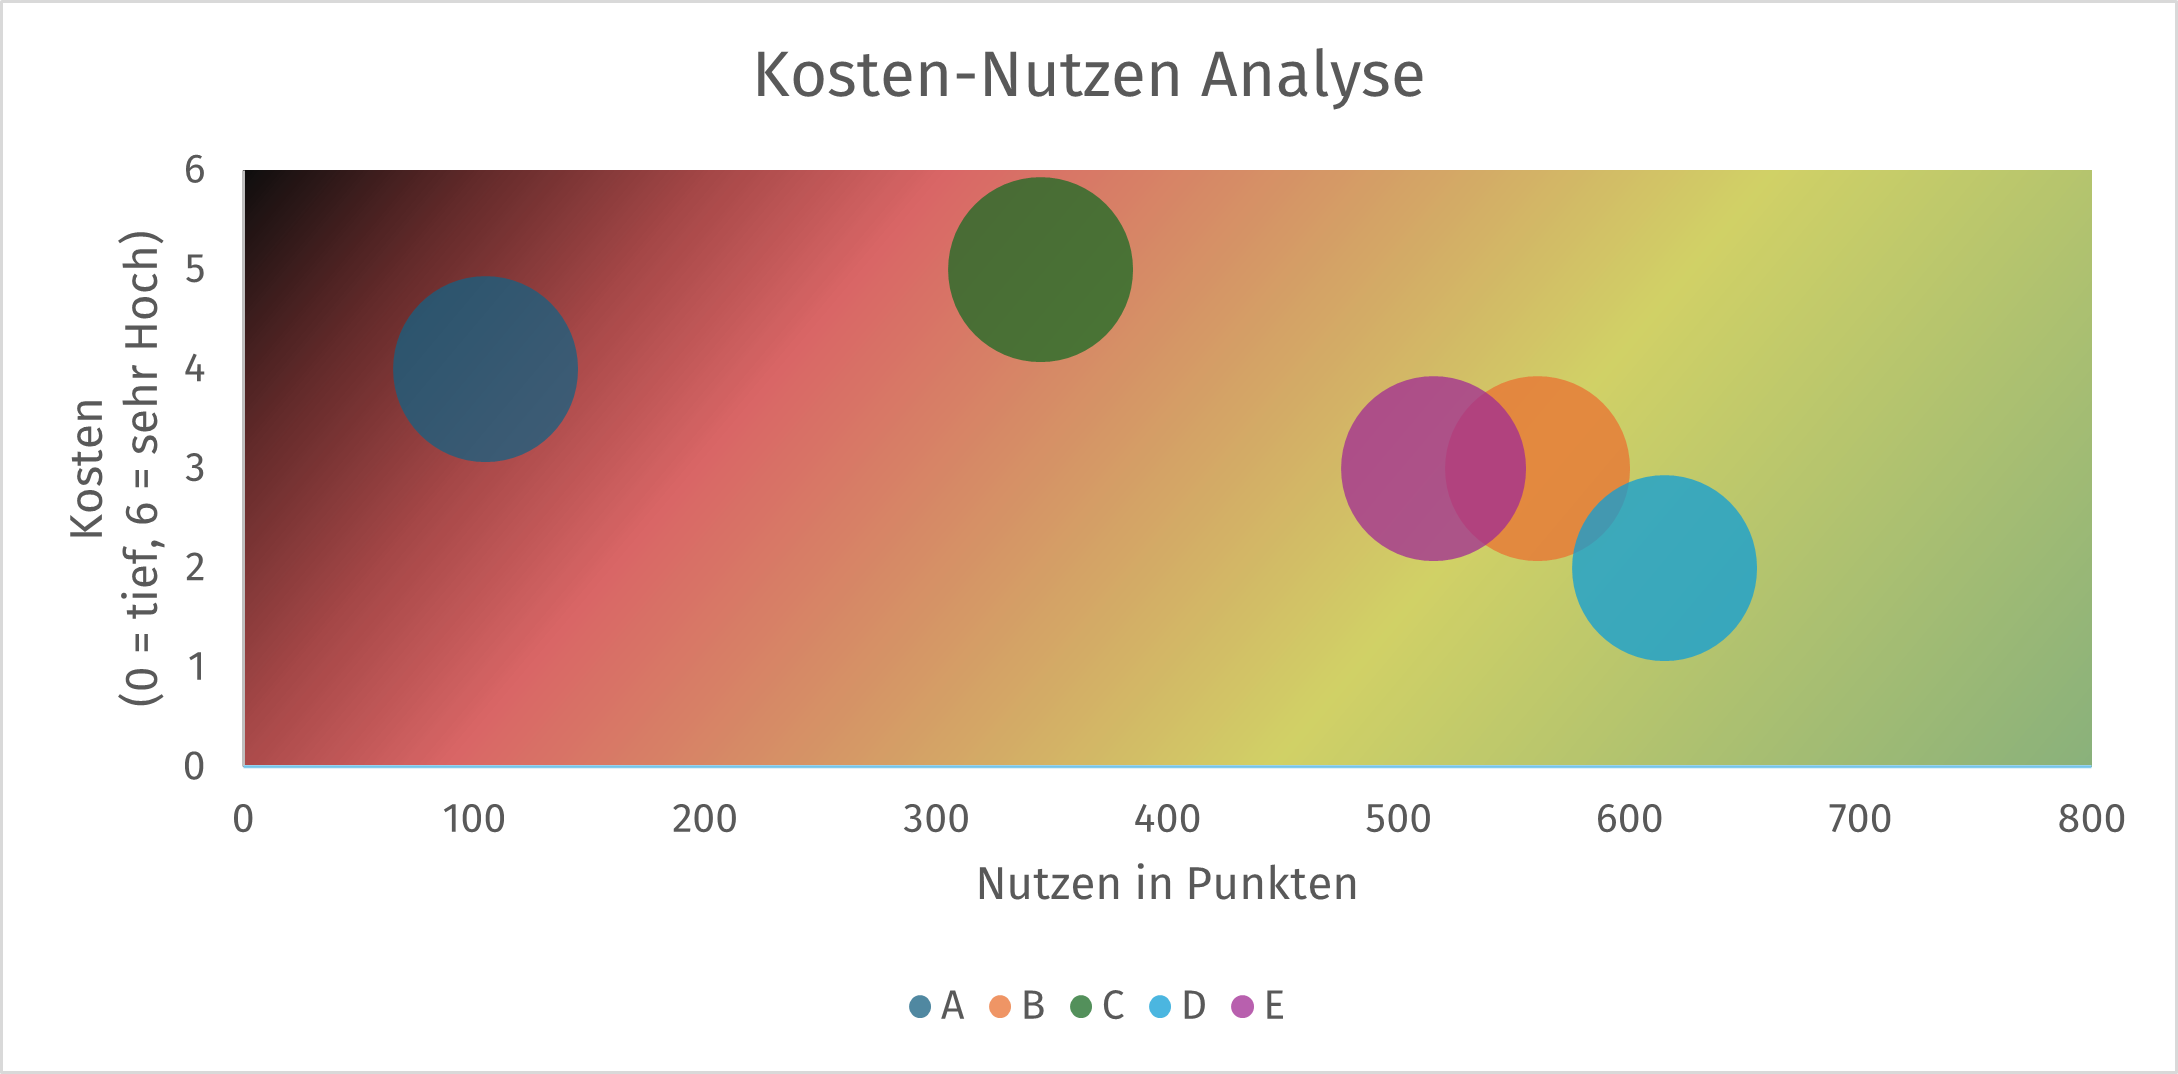
\includegraphics[width=\textwidth - 2cm]{pictures/Kostennutzenanalyse.png}
	\caption{Kosten-Nutzen Analyse}
	\label{pic:kostennutzen}
\end{figure}
\newpage
\begin{figure}[H]
	\centering
	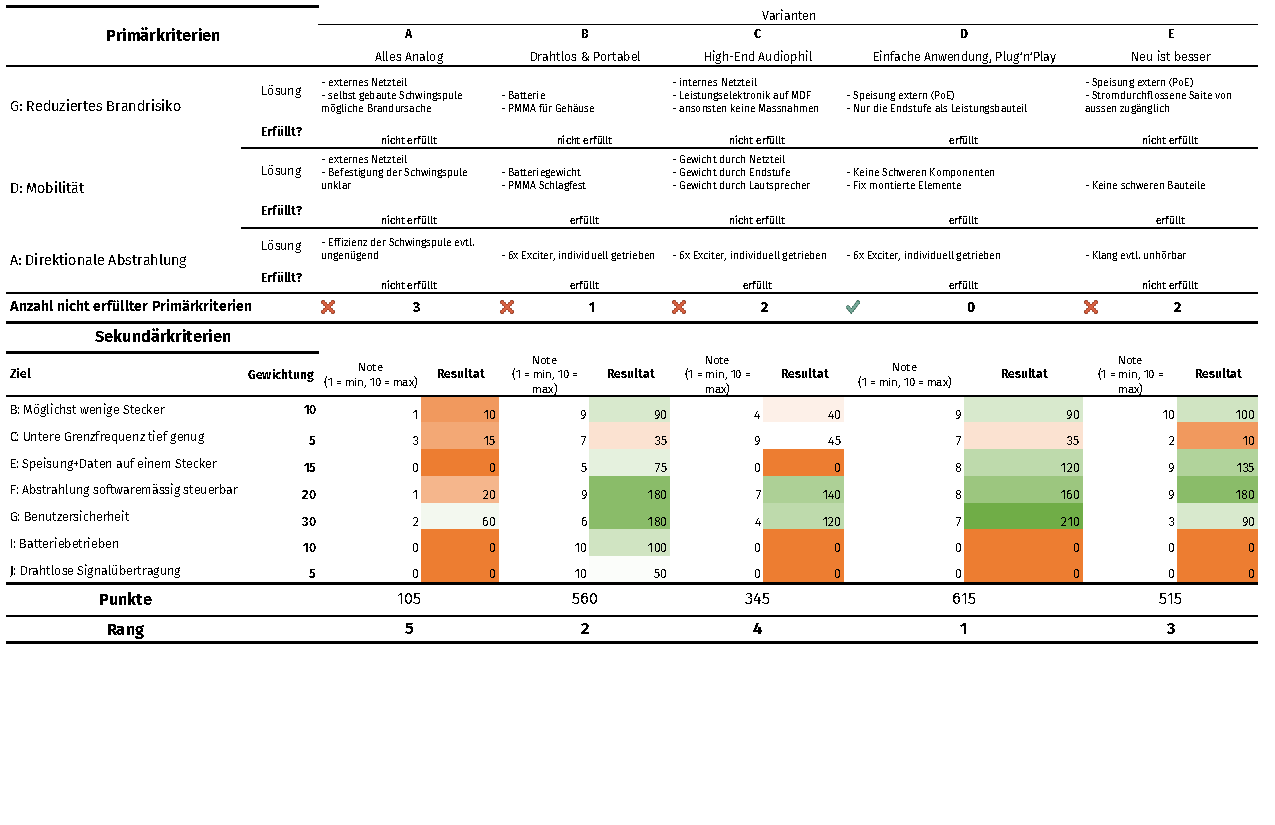
\includegraphics[trim={0 3cm 0 0},clip,width=\textheight - 1cm, angle=90]{pictures/Nutzwertanalyse.pdf}
	\caption{Nutzwertanalyse}
	\label{pic:nutzwertanalyse}
\end{figure}
\newpage